%\begin{figure*}[!t]
%	\begin{center}
%		\subfigure[No Failure]
%		{
%			\label{fig:sc_no_fail}
%			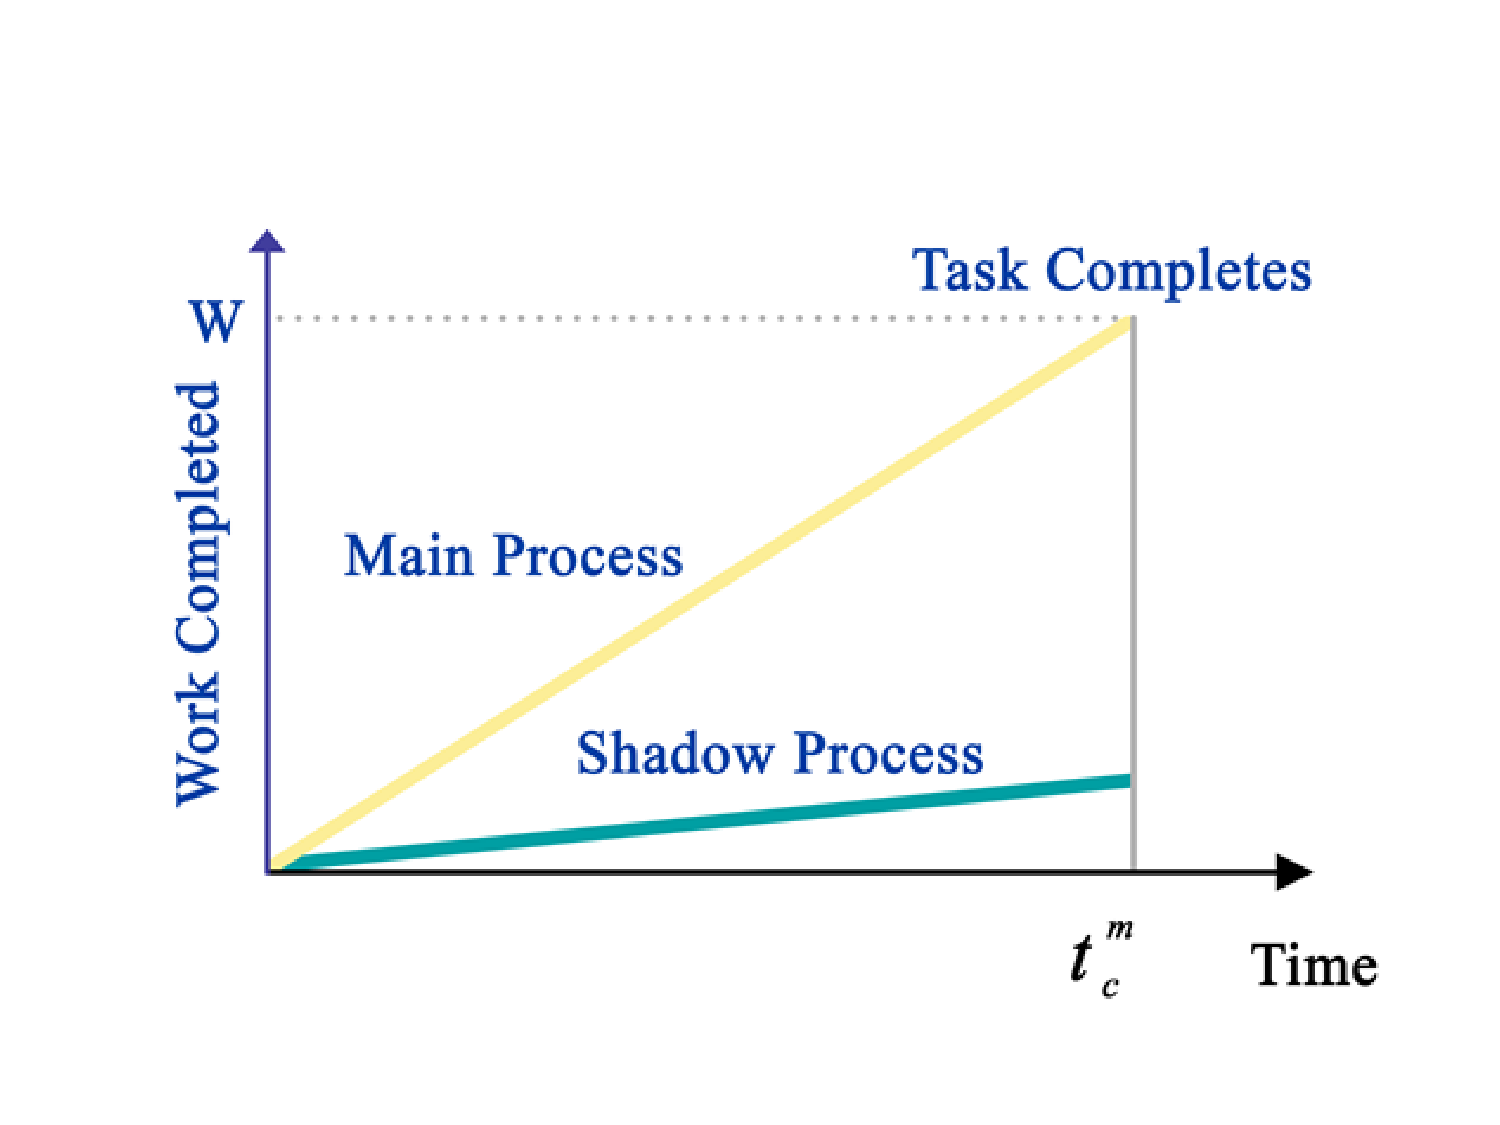
\includegraphics[width=0.32\textwidth]{Figures/example1.pdf}
%		}
%		\subfigure[Shadow Process Failure]
%		{
%			\label{fig:sc_shadow_fail}
%			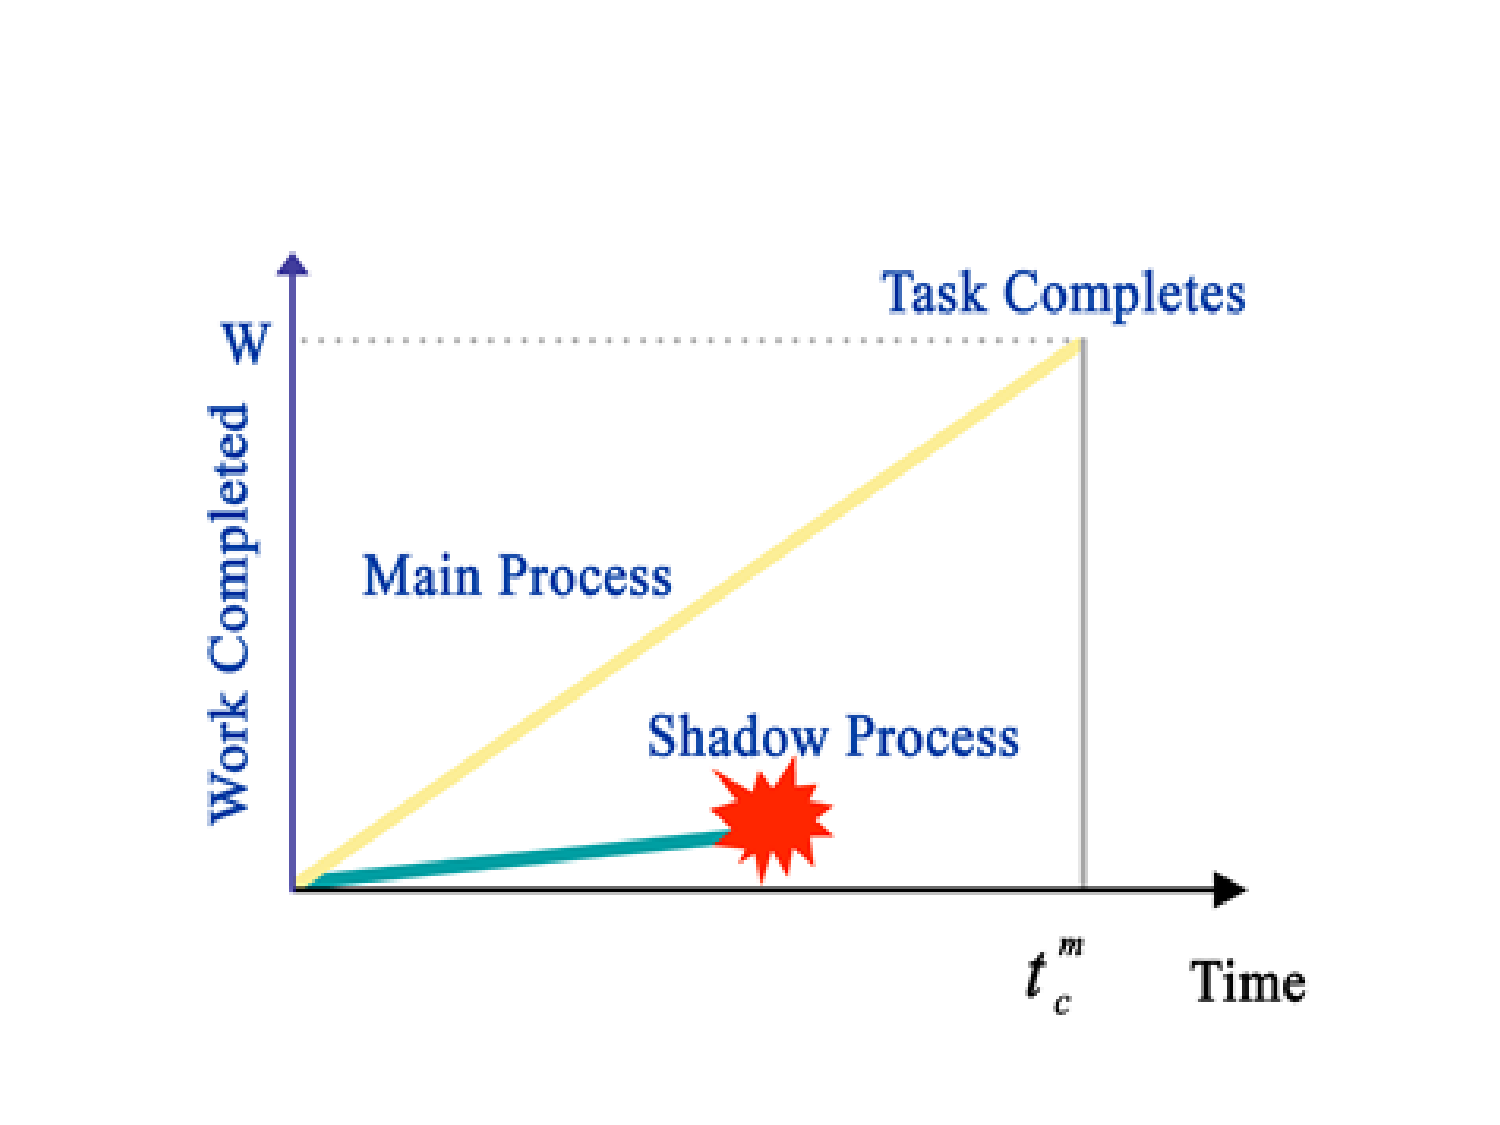
\includegraphics[width=0.29\textwidth]{Figures/example3.pdf}
%		}
%		\subfigure[Main Process Failure]
%		{
%			\label{fig:sc_main_fail}
%			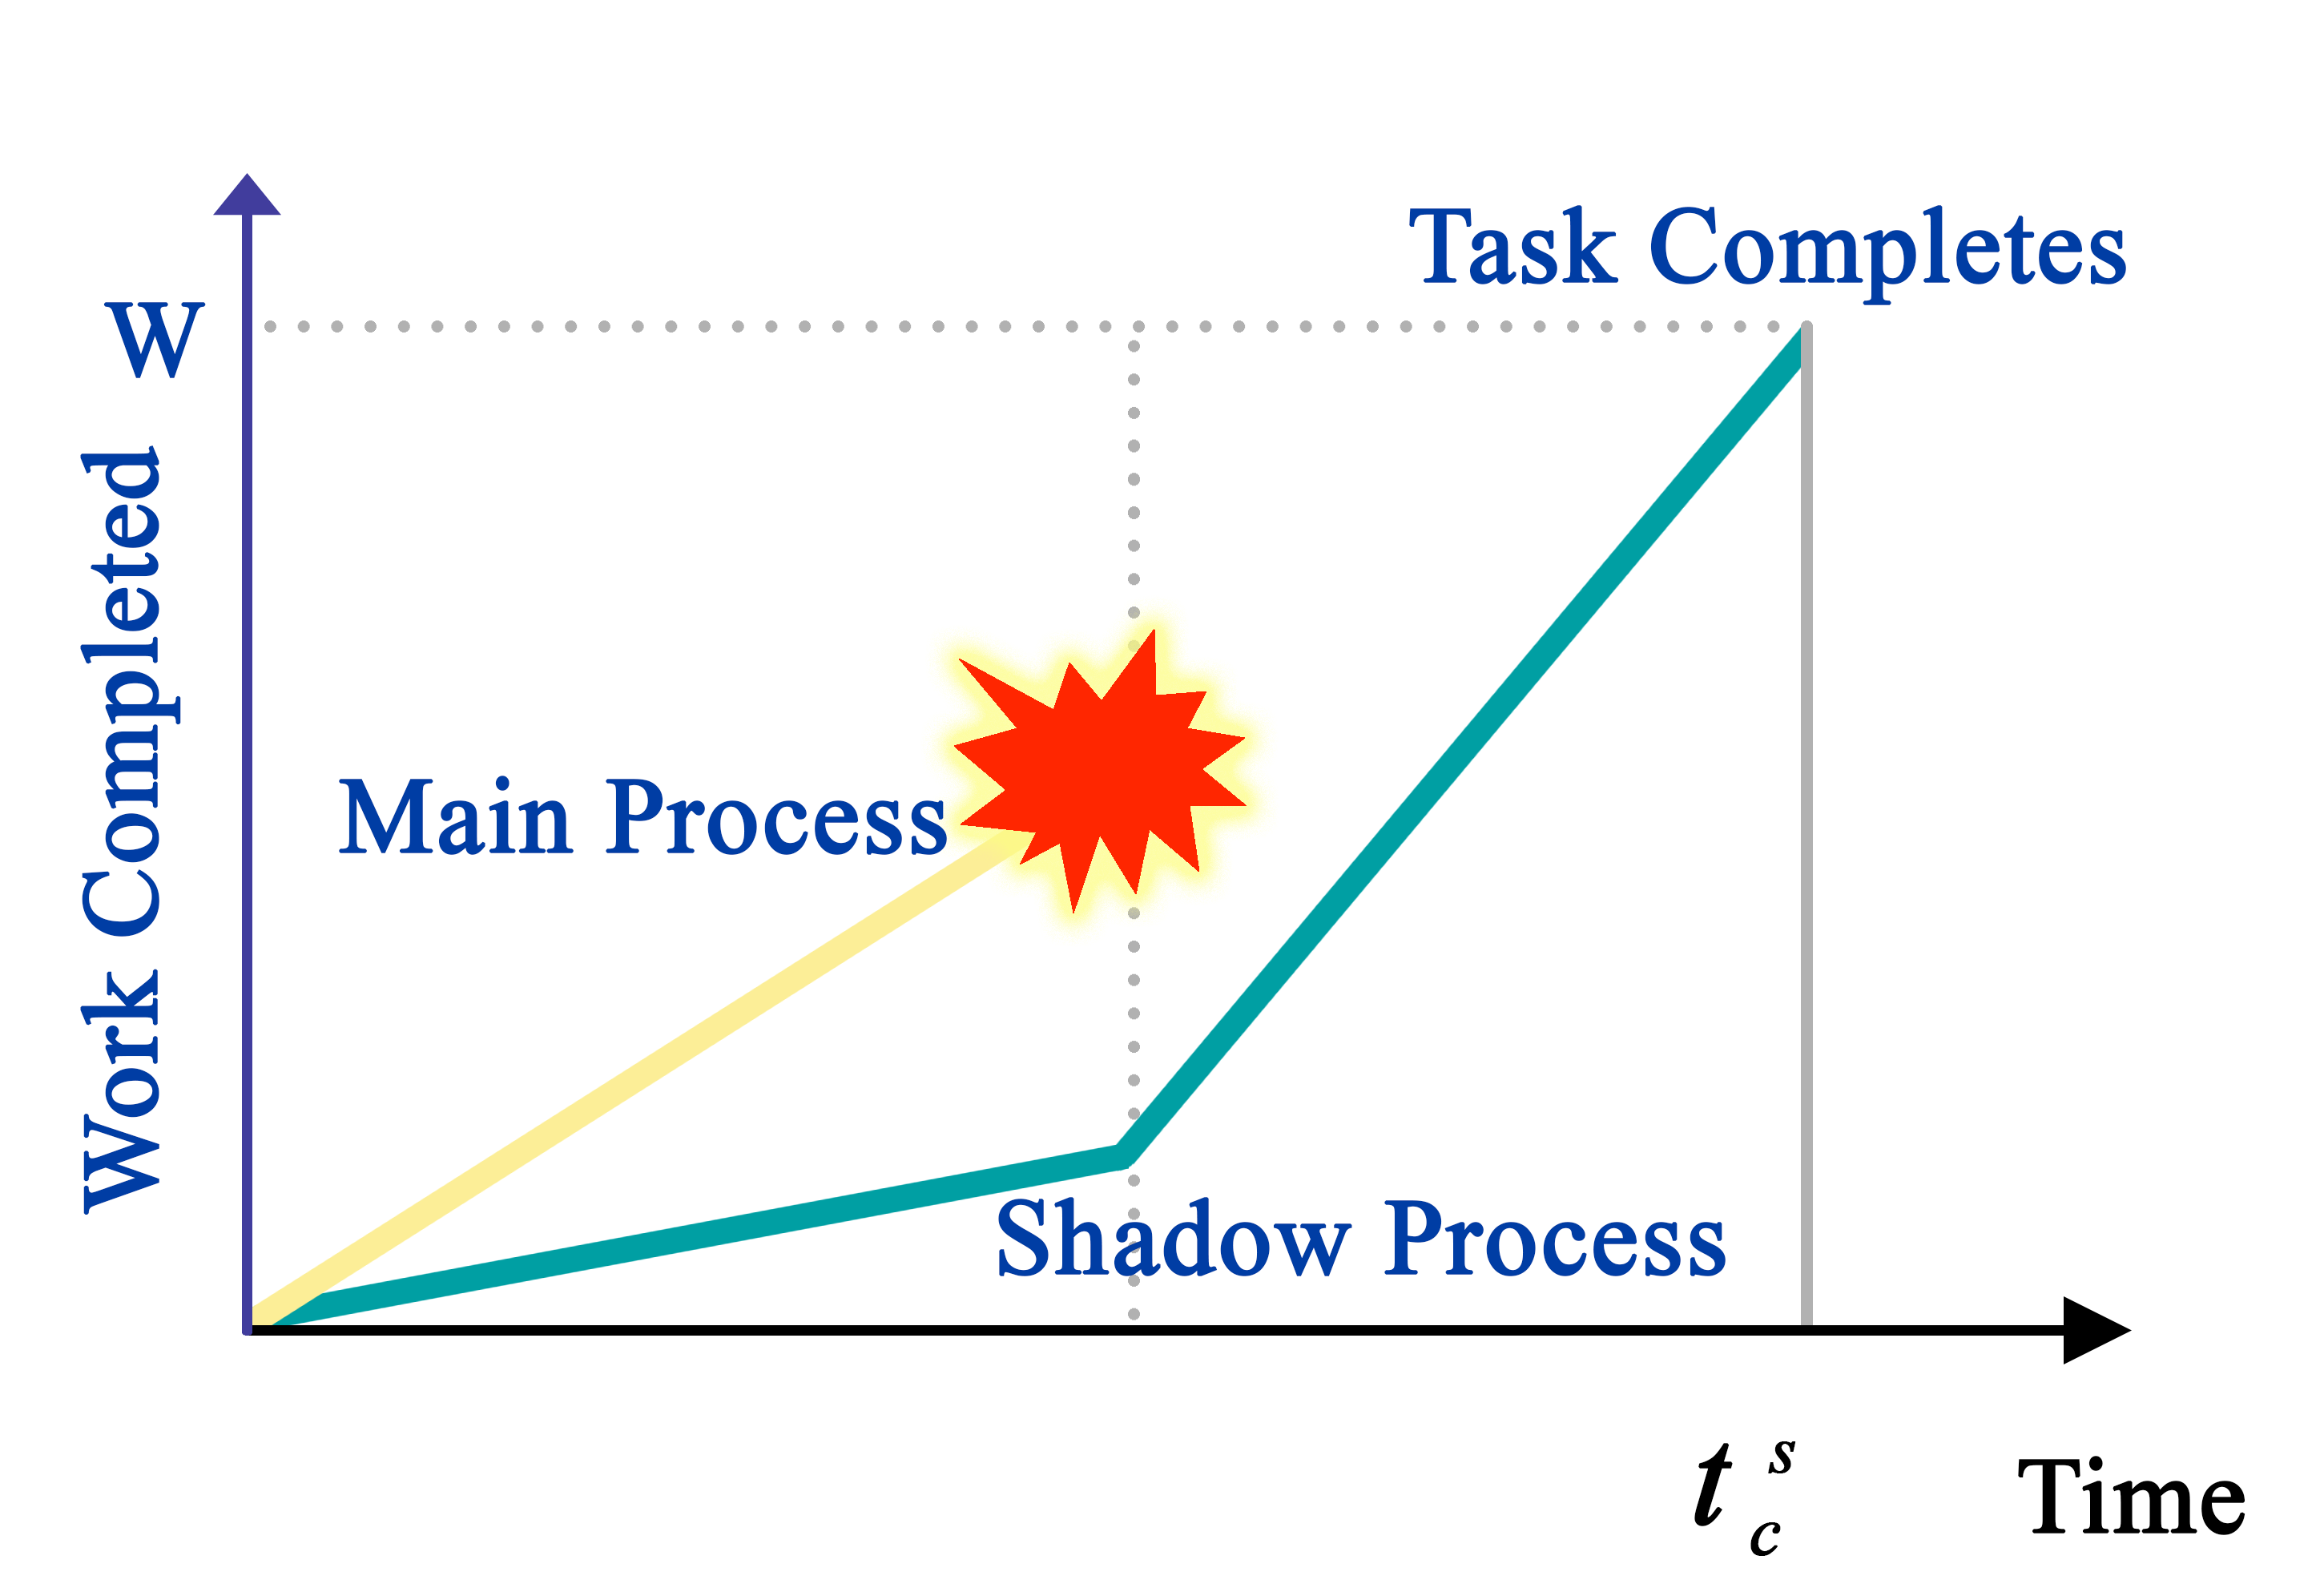
\includegraphics[width=0.33\textwidth]{Figures/example2.png}
%		}
%	\end{center}
%	\caption{Shadow Replication with a single shadow process.}
%	\label{fig:sc_overview}
%	\end{figure*}

I have been working on this research for one and a half years.
Two papers have been accepted on this work~\cite{cui_en7085151,cui_closer_2014},
and my third paper is currently under review.
Specifically, I have accomplished the following goals:
\begin{itemize}
	\item Design of a novel, scalable, and energy-aware fault tolerance framework, referred to as Shadow Replication;

	\item Development of a profit-based analytical model to explore the feasibility of
	  Shadow Replication, and to determine the optimal
	  execution rates to minimize energy and maintain quality of service (QoS);

	\item Development of an event-driven simulator to verify the above analytical model;

	\item A comprehensive evaluation using both the analytical model and simulator to analyze the
	energy savings achievable by Shadow Replication, compared to existing approaches.
\end{itemize}

%I have submitted three papers on this work. \cite{cui_en7085151} is published in Energies 7, no. 8 (2014) and \cite{cui_closer_2014} is accepted to CLOSER 2014. Our third paper is currently under review.

\subsection{Shadow Replication}
The basic tenet of Shadow Replication is to associate with each main instance a suite of ``shadows" whose size depends on the criticality of the application and its performance requirements. Each instance is executed using a process. 
To mitigate correlated failures, the main and shadow processes
execute on separate computing nodes.

%Formally, the Shadow Replication fault tolerance framework is defined as follows:
%\begin{itemize}
%	\item A main process, $P_m(W$, $\sigma_m)$, that executes at the rate of $\sigma_m$ to complete a task of size $W$;
%	\item A suite of shadow processes, $P_s(W$, $\sigma_s^b$ , $\sigma_s^a)$ $(1 \le s \le S)$, where $S$ is the size of the suite. The shadow processes %execute on separate nodes, and 
%	start execution simultaneously with the main process at rate $\sigma_s^b$. Upon failure of the main process, all shadows switch their rates to $\sigma_s^a$, with one shadow process designated as the new main process. This continues until the completion of the task.
%\end{itemize}

%Dynamic Voltage and Frequency Scaling (DVFS) is used to slow down the execution rates of the processes. 
%When DVFS is enabled, the CPU frequency (which translates to execution rate) scales proportionally to the voltage. Therefore, decreasing voltage not only reduces power and energy consumption, but also effectively slows down the running processes. 

%To illustrate the behavior of Shadow Replication, I use only one shadow process and consider the scenarios depicted in Figure \ref{fig:sc_overview}, assuming at most one process failure. Figure \ref{fig:sc_no_fail} represents the case when neither the main nor the shadow fails. The main process, executing
%at a higher rate, completes the task at time $t_c^m$. At this time, the shadow process, progressing at a lower rate, stops execution immediately. Figure \ref{fig:sc_shadow_fail} represents the case when the shadow fails. This failure, however, has no impact on the progress of the main process, which can still complete the task at $t_c^m$. Figure \ref{fig:sc_main_fail} depicts the case when the main process fails while the shadow is in progress. After detecting the failure of the main process, the shadow begins executing at a higher rate, completing the task at time $t_c^s$. Given that the failure rate of an individual node is much lower than
%the aggregate system failure, it is very likely that the main process
%will always complete its execution successfully, thereby achieving fault tolerance at a significantly reduced cost of energy consumed by the shadow. 

The novelty of Shadow Replication lies in its differentiation of the execution rates. Specifically, it 
executes the main process at the rate required for response time constraint, while slowing down the shadows for energy saving, thereby enabling a parameterized trade-off between response time and energy consumption.
A closer look at the model reveals that Shadow
Replication is a generalization of existing fault tolerance
approaches. %, namely Checkpoint/restart and Process Replication. 
Specifically, if the
QoS allows for flexible completion time, Shadow
Replication would slow down the shadow processes and trade time
redundancy for energy savings, mimicking Checkpoint/restart. %It is clear, therefore, that for a
%large response time, Shadow Replication converges to re-execution, as
%the shadow remains idle during the execution of the main process and
%only starts execution upon failure. 
If the target response time is
stringent, however, %Shadow Replication converges to process replication,
the shadows would execute simultaneously with the main at high
rates, mimicking Process Replication. The flexibility of Shadow Replication provides the
basis for the design of a fault tolerance strategy that strikes a
balance between task completion time and energy saving.%, thereby
%maximizing profit.

\subsection{Analytical model and simulator}

One challenge of Shadow Replication resides in determining
jointly the execution rates of all processes, %both before and
%after a failure occurs, 
with the objective to minimize energy while satisfying QoS requirements. To achieve this, I propose an analytical
model, from which an optimization problem is formulated to derive the optimal execution rates. The model considers the time and energy needed for a cloud job, %which is composed of multiple parallel tasks, 
under different system specifics and failure distributions. The profit is modeled as the difference between the payment from customers, which depends on the completion time, and expenses for running the cloud job, which are mainly energy costs. %Afterwards, an optimization problem is formulated to derive the optimal execution rates. 
For more details please refer to~\cite{cui_en7085151}. 

To verify the correctness of the analytical model, I build an event-driven simulator that simulates the behaviors of Shadow Replication under various configurations. It can report all necessary statistics, such as number of failures encountered, time to completion, and energy consumption. The statistics can then be used to compare with the results from the analytical model.

\subsection{Preliminary results}
Several important parameters are identified that impact the energy consumption of Shadow Replication. Correspondingly, I conduct a series of sensitivity studies where Shadow Replication is compared to state-of-the-art approaches. %The influential parameters can be classified into three categories, i.e., system specifics, SLA specifics, and job specifics. Further, the system specifics includes static power/dynamic power ratio and failure distribution, the job specifics includes workload and number of tasks, and SLA specifics is mainly targeted job completion time 
The results from both the analytical model and simulator show that Shadow Replication can achieve significant energy savings, without violating the QoS constraints. %Specifically, I conducted 4  sensitivity studies. 
Specifically, Shadow Replication can achieve 15\%-30\% energy savings under normal configurations. Furthermore, Shadow Replication would converge to Process Replication, when target response time is stringent, and to Checkpoint/restart when target response time is relaxed or when failure is unlikely~\cite{cui_closer_2014}.

%I first study the sensitivity to static power/dynamic power ratio. In this study, I considered modern systems with static power ratio from 40\% to 70\%. Within this range, Shadow Replication can achieve, on average, 19.3\% more profit than traditional replication, and 28.8\% more than re-execution. In terms of energy, the saving is 15\%-30\%.
%The second study is to the targeted job completion time. The results show that targeted job completion time influences the execution strategies of Shadow Replication to a large extent, and the reason is that Shadow Replication would strive to maintain the completion time constraint. When time is critical, Shadow Replication uses both a main and a shadow from the very beginning, in the same manner as traditional replication, to guarantee that task can be completed on time; when time is not critical, it mimics re-execution and starts its shadow only after a failure. The profit gains by Shadow Replication can be as much as 52.8\%.
%In the next study, I vary the number of tasks from 100 to 10,000,000. On average, Shadow Replication achieves 59.3\% and 18.4\% more profits than process replication and re-execution, respectively.
%Our last study is to assess the sensitivity to failure vulnerability, where I find that increasing the failure vulnerability has the same effect as increasing the number of tasks. 


%\begin{itemize}
%	\item Sensitivity to static power/dynamic power ratio. In this study, I considered modern systems with static power ratio from 40\% to 70\%. Within this range, Shadow Replication can achieve, on average, 19.3\% more profit than traditional replication, and 28.8\% more than re-execution. In terms of energy, the saving is 15\%-30\%.
%	\item Sensitivity to targeted job completion time. The results show that targeted job completion time influences the execution strategies of Shadow Replication to a large extent, and the reason is that Shadow Replication would strive to maintain the completion time constraint. When time is critical, Shadow Replication uses both a main and a shadow from the very beginning, in the same manner as traditional replication, to guarantee that task can be completed on time; when time is not critical, it mimics rexecution and starts its shadow only after a failure. The profit gains by Shadow Replication can be as much as 52.8\%.
%	\item Sensitivity to number of tasks. I considered the number of tasks from 100 to 10,000,000. On average, Shadow Replication achieves 59.3\%, and 18.4\% more profits than traditional replication and re-execution, respectively.
%	\item Sensitivity to failure vulnerability. In this study, I found that increasing the failure vulnerability would have the same effect as increasing the number of tasks. 
%\end{itemize}

%To summarize, Shadow Replication can achieve 15\%-30\% energy savings and 20\%-30\% more profit on modern systems\cite{cui_closer_2014}. Furthermore, Shadow Replication would converge to process replication, when target response time is stringent, and to re-execution when target response time is relaxed or when failure is unlikely.
